\def\fullversionflag{1}

\ifodd\fullversionflag
    \documentclass[letterpaper,11pt]{article}
\else
    \documentclass{llncs}
\fi

\usepackage{etoolbox}
\newtoggle{fullversion}
\ifodd\fullversionflag
    \toggletrue{fullversion}
\else
    \togglefalse{fullversion}
\fi

\input{latexdefs}

\iftoggle{fullversion}{
    \usepackage{authblk}
}{}

\pagestyle{plain}

\usepackage{breakcites}

\begin{document}

\title{An Introduction to Hyperledger}
\date{}
\author{Hyperledger Whitepaper Working Group}
\iftoggle{fullversion}{
}{
\institute{}
}

\maketitle


\begin{abstract}
The Hyperledger Project is a Linux Foundation sponsored initiative with the goal of building secure enterprise blockchain implementations. Hyperledger does not have a single blockchain codebase or a single blockchain project, but rather functions as an organization where projects that are accepted by the community can collaborate and share ideas, infrastructure, and even code.  In this paper we explain the reasons behind the existence of Hyperledger and some of the governance choices we made and the design philosophy we bring to projects.  We list some of the use cases and features that motivated our members to participate in Hyperledger. Additionally we outline the current state of Hyperledger in terms of the projects and development efforts that are currently ongoing, and provide directions for those looking to learn more about Hyperledger.  This paper is not intended as a technical whitepaper but rather as an introduction to Hyperledger. However, we provide appropriate references for those interested in the technical details of various aspects of Hyperledger.
\end{abstract}

\section{Introduction}
\label{sec:Introduction}
Databases and database technology have played an important part in both business and society for decades. Databases began as simple, monolithic servers. As the need for more powerful functionalities grew, things like relational databases and query languages (i.e. SQL) were invented to deal with the growing need for improved efficiency and ease of use. As the world became more connected and global, distributed databases emerged, and things like consensus algorithms and fault tolerance became popular topics in both academia and business.

Now, the world has become so interconnected that many different people and entities need to be able to use the same database(s). Traditional distributed databases typically assumed that all users were honest, and errors were the result of poor network conditions or other faults that were not due to adversarial behavior. In today's world, however, people who have competitive or even adversarial relationships with one another, even within the same entity, may need to access or edit the same information in the same database. To solve this problem, distributed ledger technology and blockchain technology were developed. The basic idea is fairly simple: with clever applications of cryptography and distributed systems concepts to traditional databases, many more useful applications can be constructed in ways that do not require a central trusted authority or reduce the trust requirements on the participants. With this in mind, we can view both blockchain and distributed ledger technology as the emerging field at the intersection of databases, cryptography and distributed systems.

Historically, databases have focused on single party applications purely out of necessity.  Since distributed databases allow for multiparty, shared database use, distributed ledgers can be equipped with multi-party business logic, which is more commonly referred to as \emph{smart contracts}.  This allows distributed ledgers to be used for substantially more applications than traditional databases.

While there are many definitions of the terms \emph{blockchain} and \emph{distributed ledger}, we will define them here for clarity. For the purposes of this paper, we refer to a \emph{blockchain} as a shared, append-only log of transactions (nothing can ever be erased or edited--only appends are allowed). We define a \emph{distributed ledger} as a multi-party, distributed database where there is no central trusted authority. When transactions are processed in blocks according to the ordering of a blockchain, the result is a distributed ledger.  In spite of our desire to clarify these terms, we will bow to popular press and use these terms interchangeably. 

Hyperledger builds on this rich technology background to bring blockchain-based distributed ledgers into a broad class of enterprise usages.  Broadly speaking, Hyperledger is an `umbrella' for open source distributed ledger platforms and related components and modules. The community of developers who participate in Hyperledger coordinate cross-industry, open source software development for projects that meet the diverse needs of those building and deploying distributed ledgers. 

The most popular existing blockchains like Bitcoin~\cite{Nak08} and Ethereum~\cite{But13} utilize completely trustless networks.  But most enterprise applications rely upon real world trust relationships that Hyperledger projects can leverage to gain efficiency, functionality, or both.

While supporting diversity of blockchain and distributed ledger technologies (necessary to meet the unique needs of enterprise applications) the consortium structure of Hyperledger also provides a means of bringing coordination from the chaos: identifying common components, avoiding duplication of effort, promoting interoperability and portability, and providing a diverse community for feedback.

In the remaining sections of the paper, we will explain what Hyperledger is and many of the design decisions and principles of the effort.

\subsection{Outline}
The rest of the paper proceeds as follows.  We start by discussing the benefits of an open source platform in section~\ref{sec:WhyOpenSource}.  In section~\ref{sec:TheUmbrellaOrganization}, we explain the umbrella nature of Hyperledger's governance structure.  We then go on to explain our design philosophy for Hyperledger in section~\ref{sec:DesignPhilosophy}.

We then move in a more practical direction.  In section~\ref{sec:RelevantUseCases}, we explain some of the interesting use cases that we expect some (or most) of the Hyperledger projects to address.  In section~\ref{sec:CurrentProjects} we list and outline each of the current top-level Hyperledger projects, and we then follow that up in section~\ref{sec:LongTermVision} with our long-term vision for the Hyperledger project.  Finally, in section~\ref{sec:Conclusion} we offer our final thoughts.


\section{Why Open Source}
\label{sec:WhyOpenSource}
"Proprietary software" refers to a commercial product licensed by a vendor, normally for a fee. It's usually sold ``as is," giving buyers no way to add unique customizations or fix bugs. Proprietary software publishers carefully guard their ``source code"---the version that a programmer can read and edit---and distribute only the run-time version that's simply a long string of numbers. 

Open source is different. This is ``software that comes with permission to use, copy, and distribute, either as is or with modifications."\footnote{ Gartner. IT Glossary. Retrieved from \url{https://www.gartner.com/it-glossary/open-source}} Open source is usually free. Since the source code is  provided, developers are free to inspect, tweak, and improve the code---and to submit enhancements back. 

\subsection{Open source is popular and reliable}
When properly designed, coded, and deployed, open source is a proven and effective choice. 

For example, the Linux operating system runs 90 percent of the public cloud workload, has 62 percent of the embedded market share, and 99 percent of the supercomputer market share. \footnote{ 2017 State of Linux Kernel Development {https://www.linuxfoundation.org/2017-linux-kernel-report-landing-page/}}

The open source \textbf{Apache web server} has been the world's most popular web server for more than 20 years, and today supports more than 40\% of all active websites. \footnote{ February 2018 Web Server Survey. Netcraft. Retrieved from \url{https://news.netcraft.com/archives/2018/02/13/february-2018-web-server-survey.html}}

Other well-known open source software includes \textbf{mySQL}---the world's most popular database server--- and the \textbf{Firefox} browser. 

\subsection{Open source has some clear benefits}
According to 2015 and 2016 annual surveys of executives and developers,\footnote{ The 10th Annual Future of Open Source Survey. North Bridge and Black Duck Software. 2016. Retrieved from \url{https://www.blackducksoftware.com/2016-future-of-open-source}} these are the key reasons why enterprises choose open source software:  
\begin{itemize}
\item Competitive features and capabilities
\item No vendor lock-in, so customers can easily switch
\item High-quality solutions
\item The ability to customize and fix bugs, through access to source code
\item Lower total cost of ownership
\end{itemize}

Some years ago, the main attraction of open source was that it was ``free." 
Today, enterprises choose open source to reduce risk, gain speed-to-market, and get a competitive edge. 
Organizations want their programmers to focus on strategic projects that add significant value---such as adding industry-specific enhancements on top of a proven platform---rather than re-inventing the wheel. 

All these benefits are heightened when an enterprise confronts any profoundly new or challenging concept---like the web in years past---and like blockchain today. 
Rather than develop an entire infrastructure and engineer all of its own solutions, enterprises can ``stand on the shoulders" of others who already did pioneering work and freely shared it with the world. 

\subsection{Open source builds trust}
Blockchain represents a perfect opportunity to benefit from open source, since the concept of trust is woven deeply into all blockchain technologies. 

Blockchain systems are engineered to enable direct, peer-to-peer transactions between parties who don't fully trust one another, or don't trust any central authority to validate transactions or mediate disputes. 
Therefore, it's essential for these parties to trust in blockchain technologies. 

We believe that an open, collaborative approach that invites participation from all stakeholders is the most effective way to build trust for enterprises---enough trust for them to widely and rapidly adopt blockchain technologies. 

\subsection{Open governance}: 
Open Governance means that technical decisions -– which features to add, how to add them and when, among others – are made by a group of community-elected developers drawn from a pool of active participants. Participation in Hyperledger through becoming a Contributor and/or Maintainer is open to anyone.

As a developer or maintainer, this translates into one thing: trust. You know how decisions will be made and the process by which people will be selected to make these decisions. Hyperledger is vendor-neutral and technical contributions are based on meritocracy. 

Companies deploying blockchain internally, and those building products and services based on Hyperledger projects, tell us they trust Hyperledger because our technologies are built in the open by a broad community. 

\subsection{Open source promotes interoperability}
``Interoperable" means that a program can talk to programs from other organizations quickly and easily. In today's connected world, this is a must-have.
And in the future, we believe that many different blockchains will support many business processes for many organizations. 

Hyperledger eases interaction across numerous blockchains. The open source Hyperledger technologies are designed from the start to support interoperability across various blockchains.  

Hyperledger Quilt is expressly focused on facilitating cross-chain transactions.

\subsection{Open source makes sense for blockchain}
Both economics and common sense are on the side of a collaborative effort like Hyperledger. 

Enterprises need robust, feature-rich, modular blockchain platforms they can tailor to meet their requirements. 
Businesses as diverse as banks, car and airplane makers, and healthcare companies make a broad ecosystem of enterprises, all cooperating with the global Hyperledger developer community.

When many different users and vendors collaborate to co-create common technologies, everyone can enjoy the proven benefits including lower risk, higher quality, and faster time-to-market. 
We believe we can do more to advance blockchain technologies by working together than by working in isolation. 
Signed-off-by: Greg Wallace <gtewallace@gmail.com>


\section{The Umbrella Organization}
\label{sec:TheUmbrellaOrganization}
Hyperledger serves as an umbrella organization that brings together users, developers, and vendors from many different sectors and market spaces. 
All these participants have one thing in common: Everyone is interested in learning about, developing, and using enterprise blockchains. 

~\newline
\emph{Here's a great place for an org chart drawn somewhat like an umbrella.---GG}
~\newline

While blockchain is a powerful technology, it is not one-size-fits-all. 
Every enterprise needs special features and modifications to help a blockchain achieve its intended purpose.
Since different organizations have different needs, there will never be one single, standard blockchain. 
Instead, we expect to see many blockchains customized with different features that provide a wide range of solutions across many industries.

Because enterprises need to understand, develop, and use many different blockchains, an umbrella organization like Hyperledger can help reduce the resources consumed by these efforts.

As the umbrella organization for open source blockchain development, Hyperledger provides these benefits: 
\begin{itemize}
\item Help keeping up with developments
\item Better productivity through specialization
\item Collaboration to avoid duplicate efforts
\item Better quality control of code
\item Easier handling of intellectual property
\end{itemize}

\subsection{Help keeping up with developments}
Navigating through all the developments in an open source environment can be daunting. 
Due to the cost and complexity involved, some organizations may give up, or never get started at all. 

Hyperledger reduces this research burden by creating a collaborative environment that streamlines communication. 
Better communication helps new participants to catch up, by gaining faster access to necessary information.
As newer participants quickly join the collaborative effort, this speeds up development, for the benefit of the entire community. 

\emph{Question: Sounds good, but how? Any concrete details we can offer?---GG}

\subsection{Better productivity through specialization}
A basic premise of economics ever since Adam Smith is that \emph{specialization}---also known as division of labor---leads to higher productivity. 
Instead of everyone doing a little bit of everything, specialization enables people to focus their energies on fewer tasks and become more expert at them. 
The benefits of specialization include more expertise, more value added, and ultimately more wealth created. 
This is why specialization has proven to be a driving factor in global economic development. 

Participants can gain the same benefits---more expertise, more value added, and better all-around productivity---by specializing in certain areas of a new technology like blockchain. 
In an open source environment that lacks any umbrella organization, this would be far more difficult. 

Hyperledger's umbrella structure encourages specialization, which yields better productivity. 
And participants who happen to specialize in similar areas aren't competing against each other. 
In an umbrella organization, specialists are encouraged to join forces to accelerate their research and development. 

\subsection{Collaboration to avoid duplicate efforts}
In a siloed environment, many people can unwittingly duplicate each another's efforts. Duplication of effort is especially negative in a new industry like blockchain, where the talent pool of seasoned developers is not yet deep. 

In an umbrella organization, collaboration between participants is highly encouraged. 
This can avoid duplication, streamline the development of new projects, and encourage the creation of common components that benefit the entire community. 

Interoperability between various distributed ledgers is also enhanced by a better understanding of other projects. 
And the governing structure provided by Hyperledger can help solve any interoperability disputes that could potentially arise. 

\subsection{Better quality control of code}
Open source software is recognized for its high quality, achieved through careful code reviews and significant debugging. 
Hyperledger promotes quality control by having a technical governing committee review all projects throughout their life cycles.  
This gives new projects a chance to be critiqued, so their developers can gain knowledge from all the existing projects. 
For their part, long-time project members may discover innovations in new projects which can enhance their own projects. 
This umbrella structure also fosters interoperability between new and existing projects.

\subsection{Easier handling of intellectual property}
Another benefit provided by the umbrella organization is easier, more consistent handling of intellectual property. 
Hyperledger frameworks and tools operate under an Apache 2.0 license for code (see \url{https://www.apache.org/licenses/LICENSE-2.0}) and Creative Commons Attribution 4.0 International license for content (see \url{https://creativecommons.org/licenses/by/4.0/}). 
Both these licenses are known to be particularly enterprise-friendly and encourage adoption. 

A single, consistent approach to intellectual property removes the need for complex and expensive contractual relationships among members. Since all participants have clearly communicated their expectations, anyone building and using Hyperledger technologies can participate without fear of running into hidden legal encumbrances.



\section{Design Philosophy}
\label{sec:DesignPhilosophy}
Distributed ledgers can have vastly different requirements for different use cases. 
For instance, when participants share high levels of trust---such as between financial institutions with legal agreements---blockchains can add blocks to the chain with shorter confirmation times due to using a more rapid consensus algorithm. 
On the other hand, when there is minimal trust between participants, they must tolerate slower processing for added security.

Hyperledger embraces the full spectrum of use cases. We recognize that different enterprise scenarios have different requirements for confirmation times, decentralization, trust, and other issues, where each issue represents a potential ``optimization point" for the technology. 

To address this diversity, all Hyperledger projects follow the same design philosophy. All our projects must be:  
\begin{itemize}
\item Modular  
\item Highly Secure 
\item Interoperable
\item Cryptocurrency-Agnostic 
\item Complete with APIs
\end{itemize}

\subsection{Modular} 
Hyperledger is developing modular, extensible frameworks with common building blocks that can  be reused.
This modular approach enables developers to experiment with different types of components as they evolve, and to change individual components without affecting the rest of the system. 
As a result, this helps developers create components that can be combined to build distributed ledger solutions well-suited to different requirements. 

This modular approach also means a diverse community of developers can work independently on different modules, and re-use common modules across multiple projects. 

The Hyperledger Architecture Working Group defines functional modules and interfaces for issues such as communication, consensus, cryptography, identity, ledger storage, smart contract, and policy.\footnote{insert link to relevant webpage or doc} 

\subsection{Highly Secure}
Security is a key consideration for distributed ledgers, especially since many use cases involve high-value transactions or sensitive data.
With large codebases, many networked nodes, and valuable data flows, distributed ledgers have become prime targets for online attackers. 
Securing a blockchain is quite a difficult task: Distributed ledgers must provide a large set of features and functions, while resisting persistent adversaries. 

Security and robustness are the keys to enable enterprise-class blockchains to evolve, and provide the critical infrastructure for next-generation business networks. 
Hyperledger projects embrace security by design and follow the best practices specified by the Linux Foundation's Core Infrastructure Initiative\footnote{insert link to relevant webpage or doc}.
As such, all Hyperledger algorithms, protocols, and cryptography are reviewed and audited by security experts as well as the wider open source community on a regular basis.

\subsection{Interoperable} 
In the future, many different blockchain networks will need to communicate and exchange data to form more complex and powerful networks. 
At Hyperledger, we believe that all smart contracts and applications must be portable across many different blockchain networks. 
This high degree of interoperability will help meet the increased adoption of blockchain and distributed ledger technologies. 

\subsection{Cryptocurrency-Agnostic}
Hyperledger projects are independent and agnostic of all cryptocurrencies and will never issue its own cryptocurrency; this is decidedly not our purpose. 
Additionally, no Hyperledger project will require a native token to provide incentives to operate the network or to manage resources. 
Howerver, the design philosophy includes the capability for tokenization that can be used for managing digital objects as well as represent currencies, depending on the purpose of the implementation, though it is not required for the network to operate.

\subsection{Complete with APIs}
All Hyperledger projects provide rich and easy-to-use APIs to allow for interoperability with other systems for easier implementation. 
A well-defined set of APIs and SDKs enable external clients and applications to interface quickly and easily with core DLT infrastructure. 
These APIs support the growth of a rich developer ecosystem, and help blockchain and distributed ledger technologies proliferate across a wide range of industries and use cases.


\section{Relevant Use Cases}
\label{sec:RelevantUseCases}
\subsection{Applying for a Loan}
\input{RelevantUseCases/applying_for_a_loan.tex}

% section name in the file
\subsection{Supply Chain: Tracking Fish from Ocean to Table}

Oceanic fishing represents more than \$ 100B in economic impact worldwide. In spite of its impact,
the industry is fraught with problems. Estimates suggest that nearly 20\% of fish are caught
illegally. In addition to the environmental impact of illegal fishing, the integrity of the industry
is also affected; a recent study based on DNA testing found that nearly $\frac{1}{3}$ of all fish
was mislabeled including 87\% of snapper and 57\% of tuna (95\% of all sushi restaurants were found
to serve mislabeled fish).

Traceability and provenance are managed in several limited domains such as Maine lobster and
Maryland crab. However, the complexity of the ecosystem (see the figure below) and its relatively
primitive use of technology limit the impact (see this article for more information on efforts to
enable traceability more broadly). Problems identified by FishWise in a 2012 study include:

Many different paths from ocean to table Lake of global authority for tracing Existing proprietary
tracing systems unscalable Most existing processes are paper-based

Oceana postulated that a shared platform for traceability would help to improve the accuracy of
labeling and reduce pirate fishing: ``Despite formidable challenges, seafood traceability is well
within reach. Simply by keeping track of where our seafood comes from at every step of the supply
chain, we can make progress against pirate fishing.''

\begin{figure}
   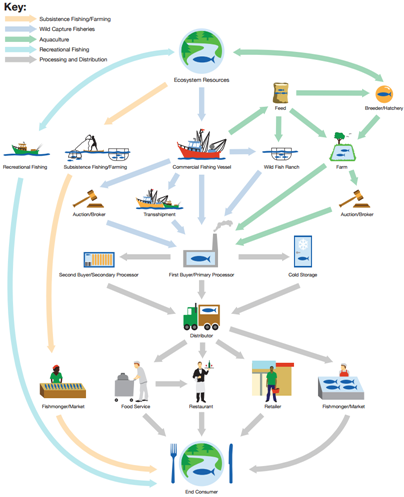
\includegraphics[scale=1.0]{figures/FishSupplyChain.png} \
   \caption{Source: \url{https://www.fishwise.org/images/fishwise_traceability_white_paper_august_2012.pdf}}
  \label{fig:supplychain}
\end{figure}

The supply chain through which fish are delivered is extremely complex (see Figure~\ref{fig:supplychain})
and involves diverse industries and regulatory controls that cross national boundaries. The
diversity of participants in the supply chain and the complex relationships between them makes this
a perfect opportunity of the use of blockchain technologies. A team at Intel is using the
Hyperledger Sawtooth blockchain technology to build a traceability prototype that combines the
distributed ledger, IoT sensors, and advanced communication technology to track telemetry parameters
such as location, temperature and humidity throughout capture, processing, and transit. Sensors
attached to the fish when it is caught record ownership and information about the location of the
catch in the ledger. Transactions on the ledger reflect interesting events in the processing of the
fish: ownership changes, transportation company, storage temperature range, etc. Further, analytics
on the ledger can be used for both regulatory enforcement and for scientific analysis of fish
harvesting and consumption.

The prototype highlights the benefits of Hyperledger Sawtooth as a platform for asset
traceability. The lightweight, highly decentralized consensus protocol in Sawtooth (``proof of
elapsed time'') is particularly well suited to the diverse, physically and organizationally
distributed ecosystem where potentially thousands of validating nodes are required. Broad
participation in the ledger reflects the cross-industry nature of the supply chain. Additionally,
asset tracking brings in a number of issues not generally seen in ledgers that focus on financial
products. For example, asset tracking requires handling of diverse data types such as the composite
format required for telemetry and environmental sensing. Transaction families in Sawtooth
accommodate domain-specific data and the transactions that operate on it, including enforcement of
data specific constraints (such as verification of the calibration of a sensor)

The use of blockchain technologies provides a number of benefits for cross-industry
traceability. Most importantly, blockchain technologies provide a means of establishing a public (to
the community of participants) and authoritative record of provenance. Its decentralized nature and
resiliency to faults enable updates from fishing boats, trucks, cold storage facilities and
restaurants. Beyond traceability, the digitization of assets (fish in this case) opens the doors for
completely new markets that might include, for example, monetization of provenance.


\subsection{Financial Services: Post Trade Activities}
The primary drivers for adoption of blockchain in financial service industry are considerations for privacy, confidentiality, and accountability. Compliance guidelines like “Anti Money Laundering” and “Know Your Customer” demand that users/customers are known and have been given clearance by their bank and/or the market infrastructure provider. These requirements drive the adoption of primarily permissioned and private blockchains. Public blockchains still carry the risk of compromising participants' confidentiality and privacy. These considerations together with very large volumes of transactions are the primary reasons that private consortium blockchains are gaining momentum in adoption of distributed ledger technology.

Among various use cases in financial services, and especially in capital markets, post trade activities is one of the prime areas, which can benefit from adoption of blockchain.

In trading post trade processing comprises all activities after the completion of a transaction. This general description is valid for all types of trading, OTC (over-the-counter)\footnote{OTC trading takes place when the trade counterparties interact directly or via brokerage services.} trading as well as trades executed at exchanges.

On a high level post-trade-processing comprises of the following operational steps:
\begin{description}
\item [Trade validation] - activities taking place directly after trade execution, mainly validation and confirmation of the actual trading activities amongst the trade participants or through exchange. 
\item [Clearing] - alignment and  matching of the actual trade instructions and confirmations across the different counterparties as well as potential netting activities. In case the counterparties have agreed on bilateral margining or the transactions are cleared through a clearing house, the counterparty/settlement risk arising between the time of concluding the trade and the time of settlement (typically 2 - 3 days) is mitigated. 
\item [Settlement] - the (legal) realization of the actual contractual obligations to reach the finality of the transaction. This includes support processes like the notification of all relevant entities affected by the transaction.
\item [Custody activities] - custodians are responsible for the safekeeping of securities. As such the positions held by the trade counterparties have to be adjusted. 
\end{description}

Besides these operational steps, post-trade-processing typically contains reporting requirements regarding the business transaction under consideration. Amongst these are counterparty internal risk reporting\footnote{The contribution of the transaction to the market and credit risk of the respective counterparts} and regulatory reporting. 

The operational steps as well as the reporting activities are in today’s setup typically a fragmented process chain spanning across a variety of departments of the respective counterparties, typically spread across a variety of entities, such as trade counterparties, brokers, settlement agents, central security depositories, clearing houses, thus resulting in a variety of interfaces. This consequently can result in a variety of reconciliation efforts along the process chain, between the trade counterparties as well as other entities/service providers involved, introducing inefficiencies in post trade processing.

Implementing post-trade-processing on blockchain is bound to lead to process efficiency gains as compared to the current implementation model. When settling via a blockchain system one could exploit the peer-to-peer property of a blockchain, i. e. one counterparty would insert the transaction details into the system and the other counterparty would verify and confirm.  Thus the confirmation processes would be processed within the same system, rendering separate confirmation processes obsolete.

In today’s world both parties would independently send their settlement instructions to a trusted 3rd party – the settlement agent – and this 3rd party would match both data sets and further process the settlement. Any mismatches in the initial instructions would lead to reconciliation efforts or even failed trades. In case of a blockchain solution, the network itself acts as an independent trusted 3rd party due to it's immutability and irrefutability of transactions.

The complexity of the multi-party interactions/interfaces is additionally reduced as all data from all from all process steps and actors resides on the blockchain and is accessible on a need-to-know basis. Therefore, the reconciliation processes should become obsolete altogether. Also the blockchain based system of record could serve as an efficient basis for reporting activities, e. g. regulatory transaction and trade reporting.

These efficiency gains have significant benefit to trade validation, clearing, both risk and regulatory reporting, as well as some aspects of the settlement phases of post trade processing\footnote{Using blockchain for near-time settlement may eliminate the netting (position offsetting) benefits to the counterparties derived from end-of-day processing, so its utility for the settlement portion of the post trade processing may be limited.}.

When looking to apply blockchain to financial services, in addition to the commonly recognized properties of a tamper-proof irrefutable transaction log, a blockchain used for post trace activity it would need to have several features, typically possible with the use of permissioned distributed ledgers.

Distributed ledgers used for capital markets use cases would typically be expected to have immediate finality. Nakamoto-style consensus algorithms (such as proof of work, proof of stake, or proof of elapsed time) may result in temporary forks, leading to transaction rollback, which is not acceptable for post trade processing use case. It is therefore expected that the blockchain applied here will have the ability to use a consensus algorithm, which has immediate finality.

Post trade activity participants have the expectation of privacy and confidentiality of transactions. The clearing house recording the transaction must ensure that parties are not able to perceive each others position and trade information. Moreover, the existence of trades themselves, even if parties are anonymized, should not be revealed since it may make transactions susceptible to traffic analysis. Current generation of analysis tools may be able to compromise both identity of the participants and trading patterns, which could be correlated to the public market information.

As described above current post trade activities happen at the end of the business day, thus presenting a different set of performance requirements than a system based on a blockchain would have. The total number of transactions would increase given the participants' ability to learn their position with the clearing house in near real-time. So while the average transactions per second number would increase, the peak performance requirements would decrease significantly.

\textbf{Hyperledger Fabric} channels combined with separate endorser sets provide an excellent solution to the problems of privacy and confidentiality. Ability to restrict data replication to only permissioned parties brings the benefits of the blockchain for data integrity and non-repudiation of transactions without compromising the security of the data. Additionally, reporting requirements - both internal and external - can be satisfied by including a regulatory agency and other oversight entities as members of the channel.

\textbf{Hyperledger Sawtooth} transaction families provide a reliable and performant way to encapsulate the operations relevant to the post trade. The ability to build complex rules using a language of choice to expose the interface which only provides the functions permitted in the context, bring a higher level of trust for the financial services institutions by providing the smart contract functionality without the risk of ad-hoc deployable code.

\textbf{Hyperledger Indy} provides an ability to have unlinkable verifiable claims, which can be leveraged to report outstanding risk on a shared ledger without compromising the identity of the firm, but still allow a regulatory body to have a holistic view of the market, enabling it to prevent potential market crashes and major defaults.


% section name in the file
\subsection{Health Records: Credentialing}

Blockchain technologies have the potential to ameliorate one of the great annoyances of modern
medical practice: ``credentialing''. Credentialing is the process a hospital uses to ensure that
its physicians are competent and worthy of the trust that patients put in them. In a sense,
credentialing is the hospital's way of performing ``due diligence'' on a physician.

A physician who wishes to become affiliated with a hospital begins the process by first gathering
copies of all of his or her professional credentials including, for example:

\begin{itemize}
\item Medical school diploma
\item Certificates of any residencies and fellowships the physician completed
\item Copies of any specialty medical boards that have certified the physician
\item All state medical licenses held by the physician
\item Evaluations from peers
\item Proof that the physician is current on continuing medical education requirements
\item Letters from hospitals with which the physician was previously affiliated, explaining the
  circumstances under which the affiliation ended 
\item Details of any malpractice actions against the physician
\end{itemize}

The hospital's credentialing office checks the physician's documentation for completeness, accuracy,
and authenticity. This is an exacting task.  Almost inevitably, they will find shortfalls, and will
ask the physician to supply missing documents. In many cases, the hospital's credentialing office
will verify some or all of the physician's submitted documentation, e.g., telephoning the
physician's medical school to confirm that the physician did indeed graduate from there.  It is not
uncommon for weeks or months to elapse as the physician and credentialing office work to satisfy the
hospital's requirements.

Once the documentation is determined to be complete, accurate and authentic, the hospital's
credentialing committee, typically composed of both physicians and administrators, sits in judgment
of the physician and decides whether or not to allow the physician to begin practicing in
affiliation with the hospital.

When using blockchain technology in any solution, several key decisions must be made.

First, will content or pointers-to-content be placed on the blockchain?  For credentialing
solutions, it might be reasonable to place publically available information (such as state medical
licensing) on the blockchain itself.  However, private information (such as peer reviews) are better
stored off the chain to guard against compromise of encryption keys and give users the ability to
remove (but not edit) information, thereby increasing trust.

Second, what is the best way to manage the identities potentially of thousands of participants?  For
ambitious credentialing solutions, this might include every hospital, every physician, every
provider of continuing medical education, and so on.

Third, what are the resource requirements, specifically storage? Credentialling solutions may
provide service for decades. Persistent commitment of participation comes with a potentially
significant contribution of resources for compute, communication, and storage. For example, what if,
a few years from now, credentialing organizations want video testimony from peers?

Hyperledger Indy provides off-the-shelf solutions for what would otherwise require careful
engineering of new software modules. Indy implements the proposed W3C standard for verifiable
claims. This capability provides a method for pairwise exchange of selected credential
attributes. For example, a physician could request a credential from their medical school that
attests to their successful graduation. That credential could be provided by the physician to a
hospital as verification of education. An important property of Indy and their implementation of
verifiable claims is that the the credential for education can be verified by the hospital as
graduation from an accredited university without the need to contact the medical school
directly. The applying physician need only expose precisely what is required for credentialing at
the hospital; no additional exposure is necessary.




\section{Current Projects}
\label{sec:CurrentProjects}
\input{CurrentProjects/current_projects.tex}

\section{Highlighted Features}
\label{sec:HighlightedFeatures}
\input{HighlightedFeatures/highlighted_features.tex}

\section{Long-Term Vision}
\label{sec:LongTermVision}
\input{vision.tex}

\section{Conclusion}
\label{sec:Conclusion}
In this paper, we have explained the rationale behind the creation of Hyperledger and our goals. We outlined why we think an open source umbrella structure seems to be the optimal governing arrangement for a general blockchain consortium. We proposed some of the use cases that inspired our members to found and develop Hyperledger and delineated some of the benefits that result from building blockchain in such an organization for some of these interesting use cases. In addition, we briefly summarized all of the main Hyperledger projects and their statuses.

While this paper is not intended to be technical, we note that there is a wealth of technical information on the Hyperledger wiki. Each of the main projects has quite a bit of documentation, getting-started guides, and help available here\footnote{If this isn't true, it should be!}. In addition, some of the working groups have great technical resources.  The architecture working group has a substantial amount of documentation on permissioned blockchain fundamentals and is a great resource for those looking to explore technical details. There are also application-specific working groups that are great places to learn. For instance, the Identity working group has spent a lot of time discussing and documenting how blockchain can enable identity solutions. We encourage readers to look to these places for more information on topics that they find interesting.   

We hope that this paper is just the beginning of the Hyperledger experience for many. We acknowledge that there is a lot of work left to be done, and that Hyperledger will almost always be a work-in-progress. However, we think our organization is solid and believe that, maybe with your help, we can build secure, efficient, and reliable blockchain solutions.


Signed-off-by: Travin Keith <travin@travinkeith.com>


\iftoggle{fullversion}{
    \bibliographystyle{alpha}
}{
    \bibliographystyle{alpha}
}
\bibliography{hyperledger}

\appendix
\section{Authors and Acknowledgements}
We as the Hyperledger Whitepaper Working Group would like to thank the following people for contributing to the writing of this paper:

Tamas Blummer, Sean Bohan, Mic Bowman, Christian Cachin, Nick Gaski, Nathan George, Daniel Hardman, Ram Jagadeesan, Travin Keith, Renat Khasanshyn, Murali Krishna, Tracy Kuhrt, Arnaud Le Hors, Stanislav Liberman, Esther Mendez, Dan Middleton, Hart Montgomery, Dan O'Prey, Drummond Reed, Stefan Teis, Dave Voell, Greg Wallace, Baohua Yang.


In addition, we would like to thank the Hyperledger Technical Steering and Marketing Committees for providing valuable feedback throughout the process of writing this paper.


\end{document}
